\documentclass{beamer}

\graphicspath{{figures//}}

\usepackage{scn-slides}

%%%%%%%%%%%%%%%%%%

\title{Лекция 10\\Представление в базе знаний соответствий}
\author[]{Шункевич Д.В.}
\institute[]{Белорусский государственный университет информатики и радиоэлектроники}

\begin{document}

\begin{frame}
	\titlepage
\end{frame}

\begin{frame}{\\Содержание лекции}
	\topline
	\justifying
	Типология соответствий. Однозначные и неоднозначные соответствия. Область определения и область значений соответствия, образ и прообраз. Отображения и биективные соответствия. Соответствия на структурах. Гомоморфизмы, изоморфизмы, автоморфизмы, представление в базе знаний.
\end{frame}

\begin{frame}{\\Типология соответствий}
\topline
\begin{SCn}
\scnheader{соответствие*}
\scnidtf{наличие соответствия*}
\begin{scnrelfromset}{разбиение}
        \scnitem{однозначное соответствие*}
	\scnitem{неоднозначное соответствие*}
\end{scnrelfromset}
\begin{scnrelfromset}{разбиение}
        \scnitem{всюду определенное соответствие*}
	\scnitem{частично определенное соответствие*}
\end{scnrelfromset}
\begin{scnrelfromset}{разбиение}
        \scnitem{сюръекция*}
	\scnitem{несюръективное соответствие*}
\end{scnrelfromset}
\end{SCn}
\end{frame}

\begin{frame}{\\Однозначное соответствие}
\topline
\begin{SCn}
\scnheader{однозначное соответствие*}
\scnidtf{наличие однозначного соответствия*}
\scnidtf{функциональное соответветствие*}
\scnidtf{функция*}
    \scnrelfrom{определение}{\normalfont{[}однозначное соответствие* – это соответствие*, при котором каждому элементу из области отправления’ соответствия ставится не более, чем один элемент из области прибытия’ соответствия.\normalfont{]}}
\end{SCn}
\end{frame}

\begin{frame}{\\Однозначное соответствие}
    \topline
    \begin{center}
        \begin{figure}[Hb]
            \centering
            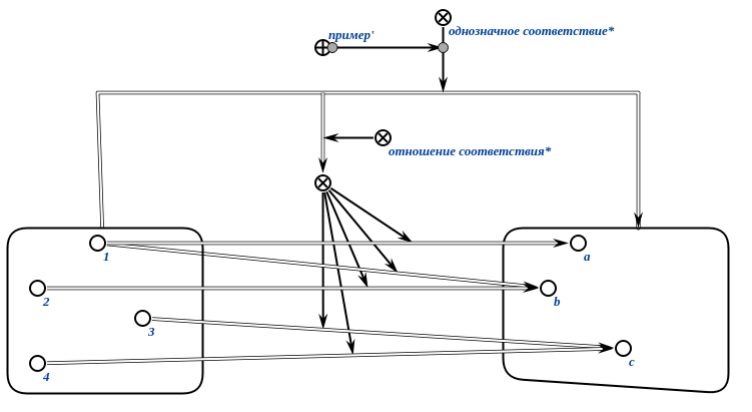
\includegraphics[scale=.72]{figures/sd_correspondences/One-to-one correspondence.png}
        \end{figure}
    \end{center}
\end{frame}

\begin{frame}{\\Неоднозначное соответствие}
\topline
\begin{SCn}
\scnheader{неоднозначное соответствие*}
\scnrelfrom{определение}{\normalfont{[}неоднозначное соответствие* – это соответствие*, при котором хотя бы одному элементу из области отправления соответствия ставится более, чем один элемент из области прибытия соответствия.\normalfont{]}}
\end{SCn}
\end{frame}

\begin{frame}{\\Неоднозначное соответствие}
    \topline
    \begin{center}
        \begin{figure}[Hb]
            \centering
            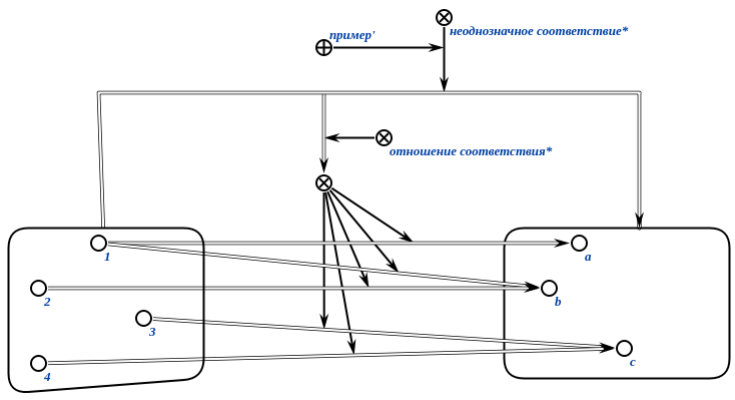
\includegraphics[scale=.72]{figures/sd_correspondences/Ambiguous correspondence.png}
        \end{figure}
    \end{center}
\end{frame}

\begin{frame}{\\Область определения соответствия}
\topline
\begin{SCn}
\scnheader{область определения соответствия\scnrolesign}
\scnidtf{область отправления соответствия\scnrolesign}
\scnidtf{первый компонент пары в отношении соответствия\scnrolesign}
\scniselement{ролевое отношение}
\scnrelfrom{определение}{\normalfont{[}область определения соответствия\scnrolesign – ролевое отношение, указывающее на первый компонент пары в рамках отношения соответствие*.\normalfont{]}}
\end{SCn}
\end{frame}

\begin{frame}{\\Область значений соответствия}
\topline
\begin{SCn}
\scnheader{область значений соответствия\scnrolesign}
\scnidtf{область прибытия соответствия\scnrolesign}
\scnidtf{второй компонент пары в отношении соответствия\scnrolesign}
\scniselement{ролевое отношение}
\scnrelfrom{определение}{\normalfont{[}область прибытия – ролевое отношение, указывающее на второй компонент пары в рамках отношения соответствие*\normalfont{]}}
\end{SCn}
\end{frame}

\begin{frame}{\\Образ соответствия}
\topline
\begin{SCn}
\scnheader{образ\scnrolesign}
\scnidtf{образ соответствия\scnrolesign}
\scniselement{ролевое отношение}
\scnidtf{второй компонент пары в отношении соответствия\scnrolesign}
\scnrelfrom{определение}{\normalfont{[}образ\scnrolesign – ролевое отношение, указывающее на второй компонент каждой пары в рамках множества пар, которое является вторым компонентом отношения соответствия*.\normalfont{]}}
\end{SCn}
\end{frame}

\begin{frame}{\\Прообраз соответствия}
\topline
\begin{SCn}
\scnheader{прообраз\scnrolesign}
\scnidtf{прообраз соответствия\scnrolesign}
\scniselement{ролевое отношение}
\scnidtf{первый компонент пары в отношении соответствия\scnrolesign}
\scnrelfrom{определение}{\normalfont{[}прообраз\scnrolesign – ролевое отношение, указывающее на первый компонент каждой пары в рамках множества пар, которое является первым компонентом отношения соответствия*.\normalfont{]}
}
\end{SCn}
\end{frame}

\begin{frame}{\\Отображение}
\topline
\begin{SCn}
\scnheader{отображение*}
\scnsubset{всюду определённое соответствие*}
\scnsubset{однозначное соответствие*}
\scnrelfrom{определение}{\normalfont{[}отображение* – однозначное, всюду определённое соответствие.\normalfont{]}
}
\end{SCn}
\end{frame}

\begin{frame}{\\Отображение}
    \topline
    \begin{center}
        \begin{figure}[Hb]
            \centering
            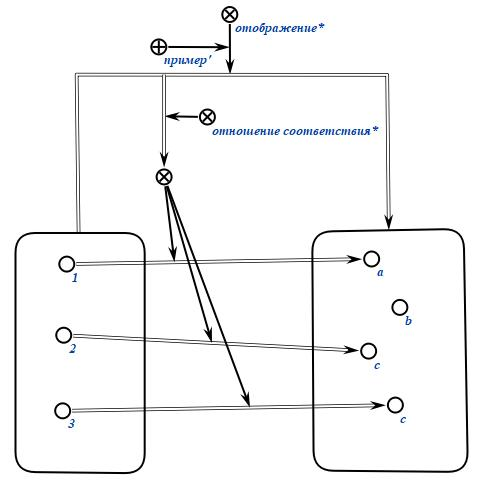
\includegraphics[scale=.45]{figures/sd_correspondences/Display.jpeg}
        \end{figure}
    \end{center}
\end{frame}

\begin{frame}{\\Биективное соответствие}
\topline
\begin{SCn}
\scnheader{биективное соответствие*}
\scnidtf{биекция*}
\scnidtf{взаимно однозначное соответствие*}
\scnsubset{всюду определённое соответствие*}
\scnsubset{однозначное соответствие*}
\scnsubset{сюръективное соответствие*}
\scnrelfrom{определение}{\normalfont{[}биективное соответствие* – однозначное, всюду определённое, сюръективное соответствие.\normalfont{]}
}
\end{SCn}
\end{frame}

\begin{frame}{\\Биективное соответствие}
    \topline
    \begin{center}
        \begin{figure}[Hb]
            \centering
            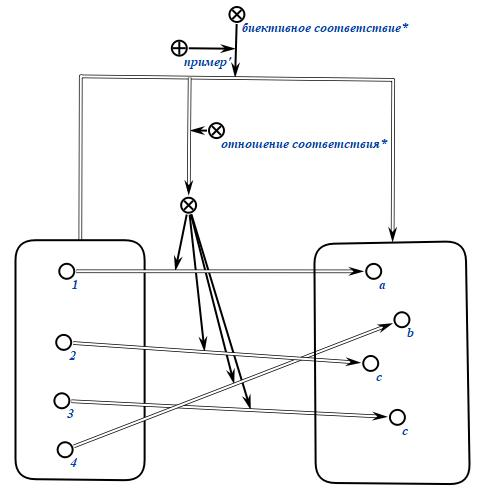
\includegraphics[scale=.45]{figures/sd_correspondences/Bijection.jpeg}
        \end{figure}
    \end{center}
\end{frame}

\begin{frame}{\\Соответствия на структурах}
\topline
\begin{SCn}
Структура – множество sc-элементов, удаление одного из которых может привести к нарушению целостности этого множества.

Между структурами можно определять ряд соответствий, таких как \textbf{гомоморфизм, автоморфизм, изоморфизм}, а также аналогичность структур, что позволяет фиксировать факт наличия некоторой аналогии,
сходства и различия некоторых подструктур рассматриваемых структур.
\end{SCn}
\end{frame}

\begin{frame}{\\Гомоморфизм}
\topline
\begin{SCn}
\scnheader{гомоморфность*}
\scnidtf{гомоморфность структур*}
\scnsubset{соответствие*}
\scniselement{бинарное отношение}
\scnrelfrom{пояснение}{\normalfont{[}гомоморфность* - это соответствие, заданное на структурах, при котором каждому элементу из области определения соответствия (первой структуры) ставится в соответствие только один элемент из области значения соответствия (второй структуры).\normalfont{]}}

\scnheader{гомоморфизм*}
\scniselement{бинарное отношение}
\end{SCn}
\end{frame}

\begin{frame}{\\Гомоморфизм}
    \topline
    \begin{center}
        \begin{figure}[b]
            \centering
            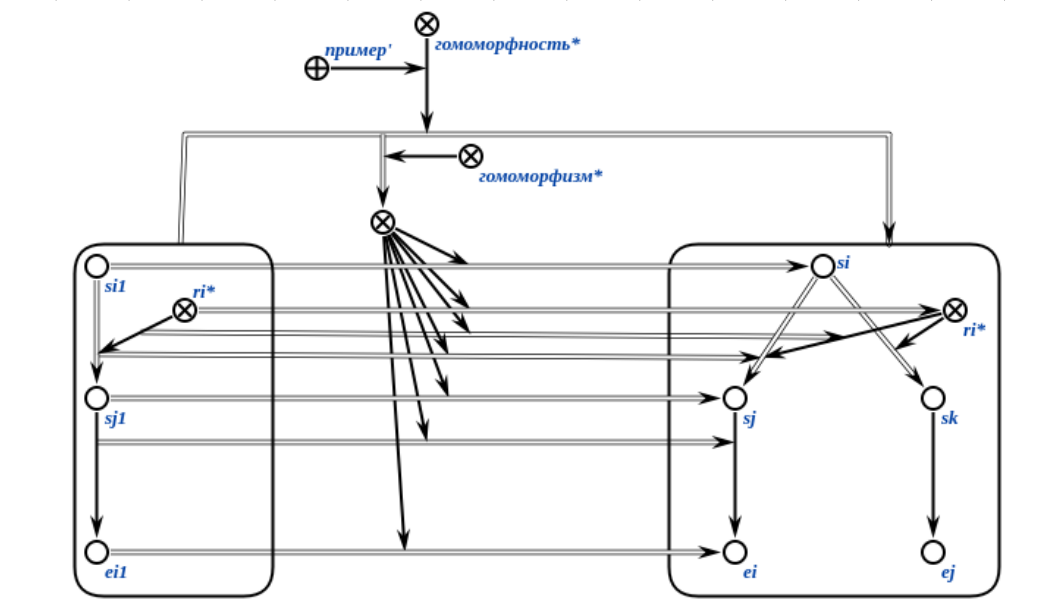
\includegraphics[scale=.45]{figures/sd_correspondences/Homomorphism.png}
        \end{figure}
    \end{center}
\end{frame}

\begin{frame}{\\Изоморфизм}
\topline
\begin{SCn}
\scnheader{изоморфность*}
\scnidtf{изоморфность структур*}
\scnsubset{соответствие*}
\scniselement{бинарное отношение}
\scnrelfrom{пояснение}{\normalfont{[}изоморфность* - это гомоморфность*, при которой для каждого элемента из области значения существует ровно один соответствующий элемент из области определения.\normalfont{]}}

\scnheader{изоморфизм*}
\scniselement{бинарное отношение}
\end{SCn}
\end{frame}

\begin{frame}{\\Изоморфизм}
    \topline
    \begin{center}
        \begin{figure}[b]
            \centering
            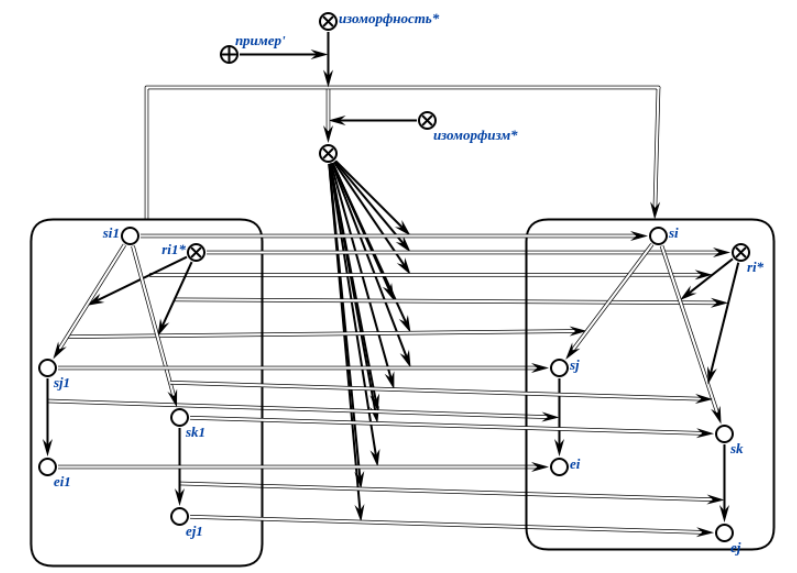
\includegraphics[scale=.5]{figures/sd_correspondences/Isomorphism.png}
        \end{figure}
    \end{center}
\end{frame}

\begin{frame}{\\Автоморфизм}
\topline
\begin{SCn}
\scnheader{автоморфность*}
\scnidtf{автоморфность структур*}
\scnsubset{соответствие*}
\scniselement{бинарное отношение}
\scnrelfrom{пояснение}{\normalfont{[}автоморфность* - это изоморфность*, у которой область определения соответствия и область значения соответствия совпадают.\normalfont{]}}

\scnheader{автоморфизм*}
\scniselement{бинарное отношение}
\end{SCn}
\end{frame}

\begin{frame}{\\Автоморфизм}
    \topline
    \begin{center}
        \begin{figure}[b]
            \centering
            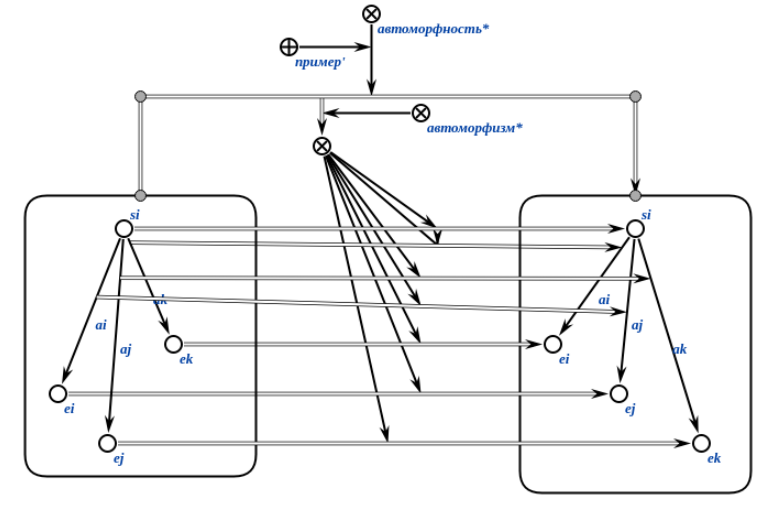
\includegraphics[scale=.55]{figures/sd_correspondences/Automorphism.png}
        \end{figure}
    \end{center}
\end{frame}

\end{document}

